\section{Introduction}

 In early 2016, Springall, Durumeric, and Halderman investigated the extent to which the site operators were reusing and sharing ephemeral values for the sake of efficiency in TLS handshakes  \cite{Springall:2016:MSH:2987443.2987480}.  Springall et. al. made TLS 1.2 handshakes over a nine week period with Alexa Top Million sites and studied the reuse of private ephemeral values in TLS session resumption, TLS session tickets, and Diffie Helmann key exchange. 
 Their key findings were surprising, demonstrating reuse of ephemeral values across Alexa Top Million websites for as long as ninety days. 

 In addition, the researchers observed more general trends such as the churn of the top million sites and protocol usage statistics. 
 Due to time constraints, the data collected spans a comparatively smaller two week period compared to the ninety day period of the original paper. 
 In the past, vulnerabilities such as heartbleed exposed between 25 and 50\% of HTTPS websites to compromise \cite{Durumeric:2014:MH:2663716.2663755}
. Thus, it is important for site operators to be aware of the security tradeoff involved in maintaining session caches for such extended periods of time. 
 
 In this paper, I revisit the original paper to reproduce a subset of these findings by collecting more data on TLS crypto shortcuts. In particular, this reproduction focuses on the usage of session ticket encryption keys and session ids by popular websites. The TLS session identifier specification (RFC 4507) describe a session state cache with unique session identifiers as keys.
 If the server supports session resumption in this manner, it will return a session id in the server hello portion of the TLS handshake. 
 On subsequent connections, previously negotiated session state can be retrieved by presenting this identifier in the client hello message \cite{RFC4507}.

The TLS session ticket extension is another way to achieve session resumption. This extension returns an encrypted block of session state to the client with an accompanying identifier for an encryption key which can decrypt this session state \cite{RFC5077}. As with session id resumption, clients can resume a session by presenting this ticket to the server in their hello message.  The session ticket extension also supports advertised lifetimes of the encrypted state.  For example, a server can specify that their session state is deleted after 5 minutes to maintain a higher degree of forward secrecy. However, even after the server has expired the encrypted state, it may still choose to reuse the encryption key identifier in subsequent tickets. 

    \begin{figure}[hp]
    \centering
    \includegraphics[height=5cm,width=\linewidth]{figures/resume_handshake.png}
    \caption{A diagram from RFC 5077 showing the abbreviated handshake for connections supporting session tickets \cite{RFC5077}. This represents a significant reduction in round trip time from the standard TLS handshake in Figure 1.}
    \end{figure}
    

The key results which I reproduce in this paper correspond to Figures 2 and 3 in the original paper. Additionally, this paper present a summary of how these TLS extension are supported across popular domains. The original paper excluded domains which did not remain in the Alexa Top Million sites for the entirety of the data collection period. The rationale behind this exclusion was that the large daily churn in this list might bias the results in favor of a large number of sites that made the list infrequently. Figure 3 quantifies this daily churn in the top sites list over the 14 day data collection period. Figure 4 demonstrates the advertised lifetimes that sites are associating with encrypted session state. 

Figure 5 show how long (in days) that session ticket encryption keys are being  reused by popular sites.  In generating this plot, this paper adopts a similar assumption to Springall et. al.
that a STEK is in use between the first and last time
that its identifier was seen and that any intermediate STEK
identifiers seen were the result of fluctuations connecting to
different servers \cite{Springall:2016:MSH:2987443.2987480}. Recall that reuse of encryption keys expose users to additional risk because it requires that the server save a copy of these keys for their lifetime. Thus, if a malicious party gains server-side access to a site which reuses keys for one week, client communications during the past week can be retroactively decrypted. 

\section{Methodology}
This data source for this analysis was collected over a continuous two week period from May 26 to June 9. As in the original paper, TLS handshakes were collected using the ZMap tool chain \cite{durumeric2013zmap}. To reduce redundant A record queries, the Alexa Top 1 Million domain names were resolved using a daily scan published to Scans.io \cite{durumericinternet}. Due to time constraints, this reproduction was limited to include the first 100K hosts in the Alexa Top 1 Million rankings. However, handshakes for all 1 million hosts over the entire 14 day period have been uploaded to this project's publicly accessible storage bucket. One implication of this choice is the difference between the resulting distributions in Figures 4 and 5. For example, higher ranked sites generally advertise lower STEK lifetimes and delete STEK identifiers more frequently. The NSS default root certificate store was used as a proxy for browser-trusted certificate. Server hellos that presented a certificate chain which was not connected to one of these roots were excluded from the results of this reproduction. 

A verbose JSON transcript of each TLS handshake used in the analysis is included in this reproduction's Google Cloud Storage bucket (identifier cs244-jared13-tls-crypto). Only a small portion of each transcript is present in this analysis; however, the scan data has been published to facilitate further analysis of TLS across popular websites without performing redundant requests. In addition, the bucket contains a summary file which only records the fields considered in the results of this paper. Subsequent analysis of the TLS transcripts were performed via Google Cloud's Compute Engine. The \href{https://github.com/jmcrawford45/cs244-final-project}{source code and setup configuration} for this analysis are published on GitHub.

\section{Results}
 
In total, 634,434 TLS handshakes were considered across 56,630 distinct domains from the Alexa Top 100K over a span of 14 days.  The common TLS connection timeout value of 72 seconds was respected in initiating handshakes. Only 24,231 domains remained in the Top 100K for the entire 14 days. Of these, 19,154 (79\%) completed a TLS handshake with a browser-trusted certificate. The distribution of the 81,750 failed connections is given in Table 1.

\begin{table}[]
\centering
\caption{The distribution of error messages when attempting to complete TLS handshakes. Connection refused messages and EOF messages typically indicate servers which do not accept connections over the TLS default port of 443. I/O timeouts represent hosts which did not respond to a TLS handshake message within 72 seconds. The majority of the handshake failure messages were due to hosts presenting a non browser-trusted certificate.}
\label{my-label}
\begin{tabular}{|l|l|}
\hline
\textbf{Error Message} & \textbf{Prevalence} \\ \hline
I/O Timeout            & 38\%                 \\ \hline
Handshake Failure      & 3\%                 \\ \hline
Other                  & 14\%                 \\ \hline
Connection Refused     & 45\%                 \\ \hline
EOF                    & 1\%                 \\ \hline
\end{tabular}
\end{table}

The original paper witnessed roughly the same proportion of consistent top 1 million hosts over the entire 90 day period. This suggests that the majority of the churn occurs below the top quintile, with sites above this rank remaining in the Alex rankings consistently. The daily churn in the Alexa Top Million website list is plotted in Figure 3. In total, over 1 million TLS handshakes were attempted. 


\begin{figure}
\centering
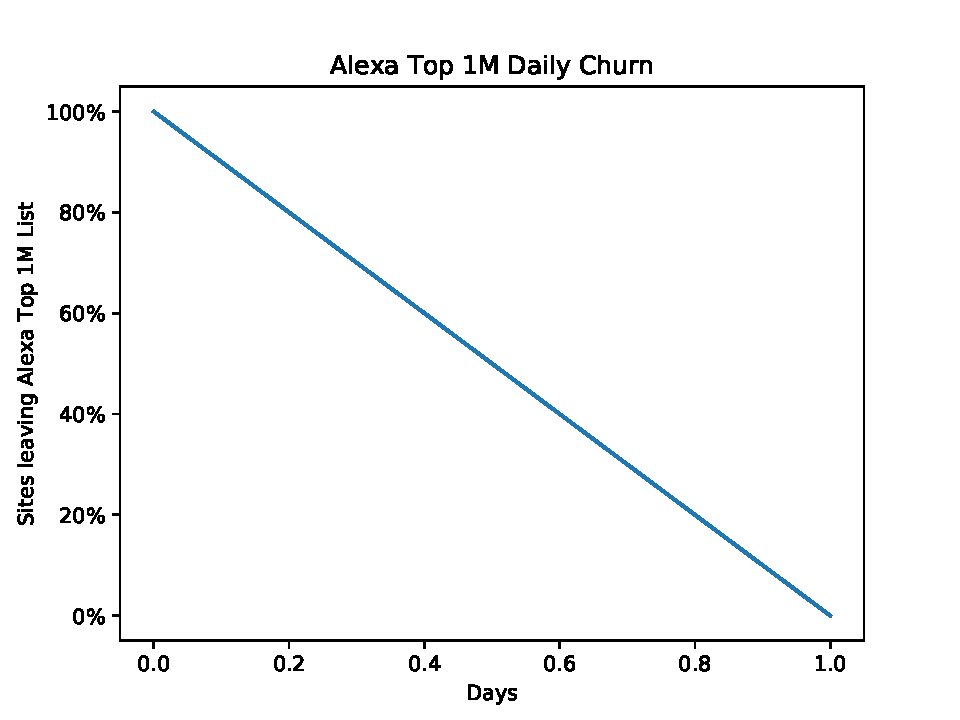
\includegraphics[width=\linewidth]{figures/churn.png}
\caption{A figure depicting the percentage of Alexa Top 1 Million hosts which are not present in the subsequent day of data collection. For example, a value of 1\% on day 5 indicates that between day 5 and 6, 1,000 IPs were not present in the subsequent A record lookups. A portion of this churn might be due to variance in A record responses across time.}
\end{figure}



\subsection{Advertised Session Lifetimes}
Servers supporting resumption via session tickets are recommended to include a lifetime advertisement, which specifies how long the server plans to honor this session ticket in storage. This allows client to remove the tickets from their cache when they expire. Figure 4 shows the distribution of these advertised values in minutes.

\begin{figure}
\centering
\includegraphics[width=\linewidth]{figures/stek_minutely_cdf.png}
\caption{A cumulative distribution plot of advertised session ticket lifetimes. Sudden spikes in the CDF likely indicate default configurations for popular deployments. The high initial value represents a combination of sites which do not support the session ticket extension or who advertise a small lifetime for STEKs.}
\end{figure}

When comparing to the data collection period of May 2016, sites in May 2018 are consistently advertising lower lifetimes for session tickets. In particular, 87\% of hosts are not advertising session tickets with lifetimes greater than 5 minutes. There is a much less prominent jump at the 18 hour mark when compared to the original paper. Springall et. al. Cloudflare as the web hosting service responsible for this large spike. Thus, it appears that Cloudflare has changed this default configuration sometime in the past two years.

\subsection{Reuse of Encryption Keys}
Of the 24,231 hosts considered, 23\% supported session resumption via session IDs and 55\% supported session resumption via session tickets.

Session ticket encryption keys were extracted from the opaque session ticket objects returned from servers supporting session resumption. The parser supported encryption key identifier extraction from a variety of open source implementations of session tickets including NSS, LibreSSL, OpenSSL, GNUTLS, and mbedTLS. The extracted key identifier corresponds to the key\_name field in the recommended ticket structure from RFC 5077 \cite{RFC5077} : 

\begin{verbatim}
    struct {
          opaque key_name[16];
          opaque iv[16];
          opaque encrypted_state<0..2^16-1>;
          opaque mac[32];
      } ticket;
\end{verbatim}
All open source implementations except mbedTLS, which uses a four byte key identifier, followed this recommendation. The original paper exploited vulnerabilities in Microsoft's Data Protection API structure to extract secrets. The parser for this reproduction does not extract encrpytion keys from this type of session ticket which is generated by Microsoft's SChannel implementation. Due to the opaque nature of the tickets returned, it is difficult to estimate the degree of coverage across different implementations of TLS. It could be the case that less widely deployed implementations have varying degrees of ephemeral value reuse. However, accounting for the most popular implementations at least provides a lower bound on ephemeral value reuse.
\begin{figure}
\centering
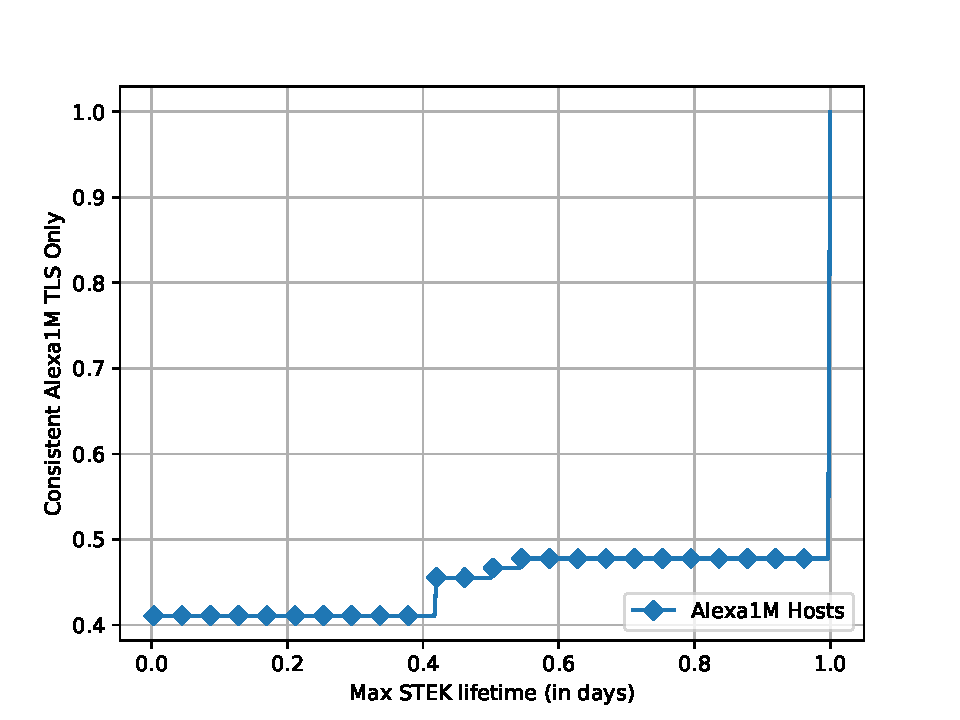
\includegraphics[width=\linewidth]{figures/max_stek_cdf.png}
\caption{A cumulative distribution plot showing the maxed observed lifetime for a session ticket encryption key (STEK). An alternative measurement of STEK reuse would be the maximum continuous interval of identical STEKs; however, the maximum lifetime of any one STEK for a host better accounts for jitter in A record responses.}
\end{figure}

The difference between the distribution in Figure 5 of this reproduction and Figure 3 in the original paper is significant. In this reproduction, almost no hosts were witnessed reusing STEK identifiers for more than 2 days. There are a few possible explanations for this discrepancy. The first, and most likely, is that the parser for this reproduction does not supply sufficient coverage over session ticket formats. As noted before, the parser does not extract STEKs from SChannel implementations of TLS, and the parsing logic for open source implementations was not thoroughly tested. An additional possibility is that the maximum discontinuous lifetime metric will simply be much larger over the span of 90 days than over 14 days. Finally, it could be the case that the top 100K hosts considered have significantly shorter lived STEKs than the entire Alexa Top 1M considered by Springall et. al.

Another concern about a plot such as Figure 5 is that it might be an inaccurate representation of the state of STEK reuse. Web traffic across the top websites roughly follows a power law or Pareto probability distribution (i.e. the majority of web traffic in the world occurs in the top 1\% or 10\% of site). To address this concern, figure 4 in the original paper provided a more stratified representation of STEK reuse differentiated by Alexa rankings. However, such a plot is not included for this reproduction as only the top 100K hosts are considered.

\section{Discussion and Future Work}
As the original paper demonstrated, mechanisms for session resumption can be weak points in TLS deployments. The TLSv1.3 draft provides better alternatives for session resumption than the TLSv1.2 session id and session ticket extensions considered in this paper. Although TLSv1.3 currently represents a negligible portion of secure transport layer traffic, analysis of ephemeral value reuse in the protocol will be necessary once the standard is more widely deployed.

Mechanisms for session resumption are a prime example of a fundamental tradeoff between security and usability. Since each application has its own latency and forward secrecy priorities, there is no single ephemeral reuse policy that is acceptable for all site operators. Thus, the original paper along with this reproduction aim to increase awareness among site operators of the prevalence and tradeoffs associated with ephemeral value reuse so that they can make the right decisions at their endpoints.
